\section{Task 1}
\label{sec:task1}

\subsection{Overview}
\label{subsec:desc1}

The first scenario tackles an interesting multi-agent coordination task, the 
distribution of robots in space.

As described in the overview of Chapter \ref{chap:experiments}, in which are 
provided additional details, in a \gls{1d} environment are spawn in a ``single 
file'' N robots in random positions. %% FIXME within the proximity sensors range 
Each agent can update its state – its absolute position – by performing actions – 
moving forward and backwards along the x-axis – based on the observations 
received from the environment – the distances from neighbours – using their 
sensors.  They are also able to transmit and receive a communication value to 
peer robots within a range of about $48$\gls{cm}. 
A full explanation of how communication works for Thymio II is covered in 
Section \ref{subsec:thymiocomm}.

As a consequence of a \gls{1d} environment, the agents' movement are 
limited to two directions: moving towards the x-axis when the velocity is positive 
while going backwards when the speed is negative. 

The robots share a common goal: arrange themselves uniformly along the 
line between the two ``dead'' robots, in such a way they stand at equal distances 
from each other.

%% FIXME The problem presents a collaborative goal given the fact that the 
%%single 
%% agent can’t sense all the environment and the final configuration depends 
%%on 
%% the position of all of them.

This problem represents a cooperative goal that can be reached performing 
imitation learning, that means training an end-to-end \gls{nn} by following 
the example of an omniscient controller, introduced in Section 
\ref{subsubsec:omniscient}.
Exploiting its complete knowledge of the environment, % FIXME state of the 
%system 
the expert is then able to decide the best action to perform.

In the course of this study, we tried to understand if it is possible to use a 
controller learned by imitation, instead of using a manual one. In particular, we 
concentrate on two approaches, presented in Sections \ref{subsec:dist} and 
\ref{subsec:comm}.
In both cases, we train \glspl{dnn} that receive sensor inputs and produce 
commands for the motors, but for the second alternative, the network has an 
addition input – the received communication transmitted by the nearest agents in 
the previous timestep – and an extra output – the message to be sent.


%%FIXME
%In this work, we decided to define and implement two multi-agent scenarios in 
%which N agents have a common goal and that requires them to coordinate 
%themselves to achieve it. Besides being an excellent example of distributed tasks, 
%the two problems present an important difference. The first is possible to solve 
%without communication, that can help to reach a more efficient solution but it is 
%not strictly necessary. The second, instead, is impossible to solve without explicit 
%communication between the agents.

\subsection{Controllers}
\label{subsec:controllers}

\subsubsection{Expert controller}
\label{subsubsec:omniscient}

As disclosed in Section \ref{sec:controllers}, the first element involved in an 
imitation learning problem is an omniscient controller, also called expert.

%fixme frase poco chiara alla fine
This controller perceives the environment and the observation of all the agents, 
obtaining a global knowledge of the state of the system. In this way it can use all 
the available information that it owns to decide the best action to perform for all 
the agents. 

In this first scenario, the omniscient controller, based on the current poses of the 
robots, moves the agents at a certain speed to reach the target positions. In 
particular, the linear velocity of each agent is computer as a ``signed distance`` 
between the current and the goal position of the robot, along its theta. 

Formally, given the current pose, defined by the triple $(x, y, \theta)$ and the 
target pose $(\overline x, \overline y, \overline \theta)$, the signed distance $d$ 
is computed as follow:
\begin{Equation}[!htb]
	\centering
	\begin{equation}
	d = \left(\overline x * \cos (\theta) + \overline y * \sin (\theta)\right) -
	\left( x * \cos (\theta) + y * \sin (\theta)\right)
	\end{equation}
	\caption[Signed distance.]{Signed distance function.}
	\label{eq:signeddist}
\end{Equation}

\noindent
To obtain the final velocity of the agent, this quantity is multiplied by a constant, 
we choose $10$ to keep the controller as fast as possible, and then clipped to its 
maximum value.

This controller can be informally considered as a simple Bang Bang controller 
since the optimal controller move at maximum speed the robot towards the target 
unless the target is closer than %%FIXME è control step o control step duration?
\texttt{control\_step\_duration} $\times$ \texttt{maximum\_speed}. In this case, 
the agent is moved lower then the maximum allowed speed so that at the end of 
the timestep it is located exactly at the target.

Unfortunately, using an omniscient controller to solve this kind of problems is not 
realistic nor feasible in a real environment.

\subsubsection{Manual controller}
\label{subsubsec:manual}
%%FIXME
The second controller we want to discuss/write about is the manual one, whose 
main purpose is to draw conclusions about the quality of the controller learned.

The main difference between this and the previous controller is that, the manual 
one can be consider a local distributed controller, that has only a partial 
knowledge of the environment since knows only the state of the current agent 
and its observations.

This controller moves the robots towards the target by minimising the difference 
between the values recorded by the front and rear sensors, trying to maintain the 
maximum achievable speed.

For each agent the controller is the same and given the same set of observations 
as input the output will be the same.

The one implemented is a proportional controller, a particular variant of \gls{pid}, 
with only the $K_p$ term. 
The closed-loop control uses a feedback to adjust the control while the action 
takes place in proportion to the existing error. This function given a desired 
output $x(t)$, or set point, produces an output $y(t)$, or process variable, such 
that the error $e(t)$ is obtained as the difference between the value of the set 
point and the process variable. Finally, the control variable is the $u(t)$ is the 
output of the \gls{pid} controller and is computed as follows:

\begin{Equation}[!h]
	\centering
	\begin{equation}
	u(t) = K_p * e(t)
	\end{equation}
	\caption[Proportioal PID controller.]{Proportional \gls{pid} controller.}
	\label{eq:pid}
\end{Equation}

The value of the proportional gain has been tuned to yield satisfactory 
performance so that the system is stable, as shown in Figure \ref{fig:pid}. 
Moreover, since the value of the error is computed using the Equation 
\ref{eq:systemerror}, then $K_p$ should be positive.

\begin{Equation}[!h]
	\centering
	\begin{equation}
	e(t) = x(t) - y(t)
	\end{equation}
	\caption{Calculation of the error value $e(t)$ of the system.}
	\label{eq:systemerror}
\end{Equation}

\begin{figure}[htb]
	\centering
	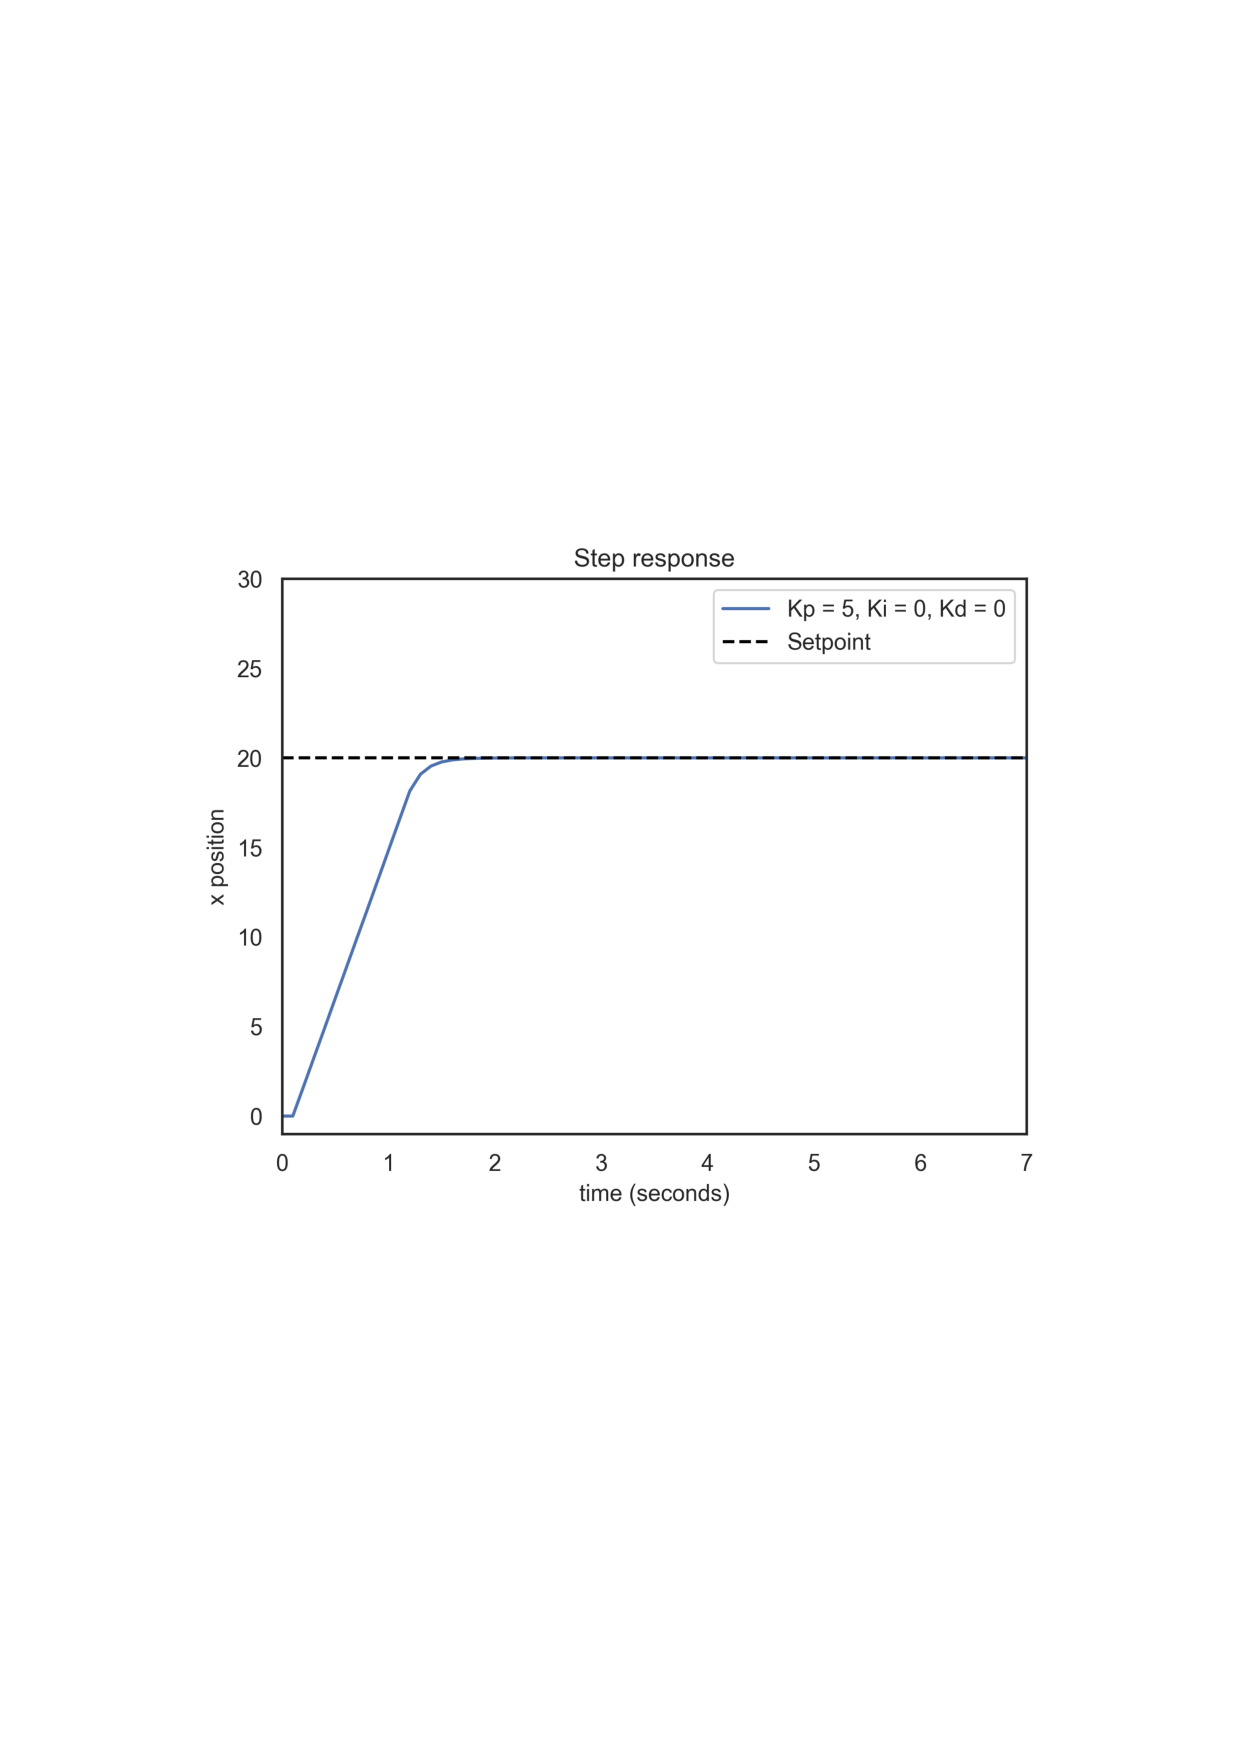
\includegraphics[width=.5\textwidth]{contents/images/Step-responsep=kp5ki0kd0}
	\caption[Step response of the proportinal PID controller.]{Visualisation of the 
	step-response of a P controller with proportional 
	gain $5$.}
	\label{fig:pid}
\end{figure}

It is important to notice that the speed returned by the controller is used to set the 
\texttt{motor\_\{left, right\}\_target}, both with the same value in order to move 
the robots straight ahead. Moreover, the first and the last robots of the line, which 
are those which sensors never receive a response respectively from the back and 
from the front, never move.

%%FIXME
See \url{https://youtu.be/jNkt7xf6pUU} for a short video that shows the 
simulation of this task \cite[][]{task1manual}.

\subsection{Distributed approach experiments}
\label{subsec:ex1distr}
\subsubsection{Learned controller}
\label{subsubsec:learneddist}

Once, enough data are collected through the simulator by using the optimal 
controller, it is possible to train a very simplified ``distributed network'' 
that takes as input an array containing the response values of the sensors – 
which can be either \texttt{prox\_values}, \texttt{prox\_comm} or 
\texttt{all\_sensors} – and produces as output an array containing one float 
that represents the speed of the wheels, which is assumed to be the same 
both right and left.

The dataset then contains a fixed number of simulation runs, each of these 
composed by a variable quantity of timesteps. It is important to notice that 
for this approach, unlike the one with communication, it is not necessary to 
keep the order of the sequence of timesteps, neither to know the exact 
number of agents in the simulation since the network input is the sensing 
associated to a single robot.

For this reason, the model is independent of the number of agents and 
consequently it is possible to prove its generalisation capacity, regardless 
the number of robots, by training the networks first on datasets each with a 
different but fixed value of $N$ and then on simulations composed by a 
variable $N$.
It is easy to show that although the value of $N$ changes the network 
structure does not, as it is sufficient during the input preprocessing to 
change the dimension of the input in such a way that all the tensors have a 
the same length, fixed at the maximum possible value of $N$, padding 
those tensors with a lower number of agents.

Thanks to these two assumptions, it is possible to shuffle the original 
dataset, based on the single run, in order to improve the generalisation on 
the samples, and then split the resulting collection into the train, the 
validation and the test sets, containing respectively $60$-$20$-$20\%$ of 
the data. 

The architecture of the network, displayed in Figure 
\ref{fig:singlenetdistributed1}, is straightforward: there are three linear 
layers each of size $\langle\mathtt{input\_size}, 10\rangle$,  $\langle 10, 
10\rangle$ and $\langle 10, 1\rangle$, where \texttt{input\_size} is the 
shape of the sensing, that can be $7$ or $14$.

\begin{figure}[htb]
	\centering
	\begin{subfigure}[h]{0.495\textwidth}
		\centering
		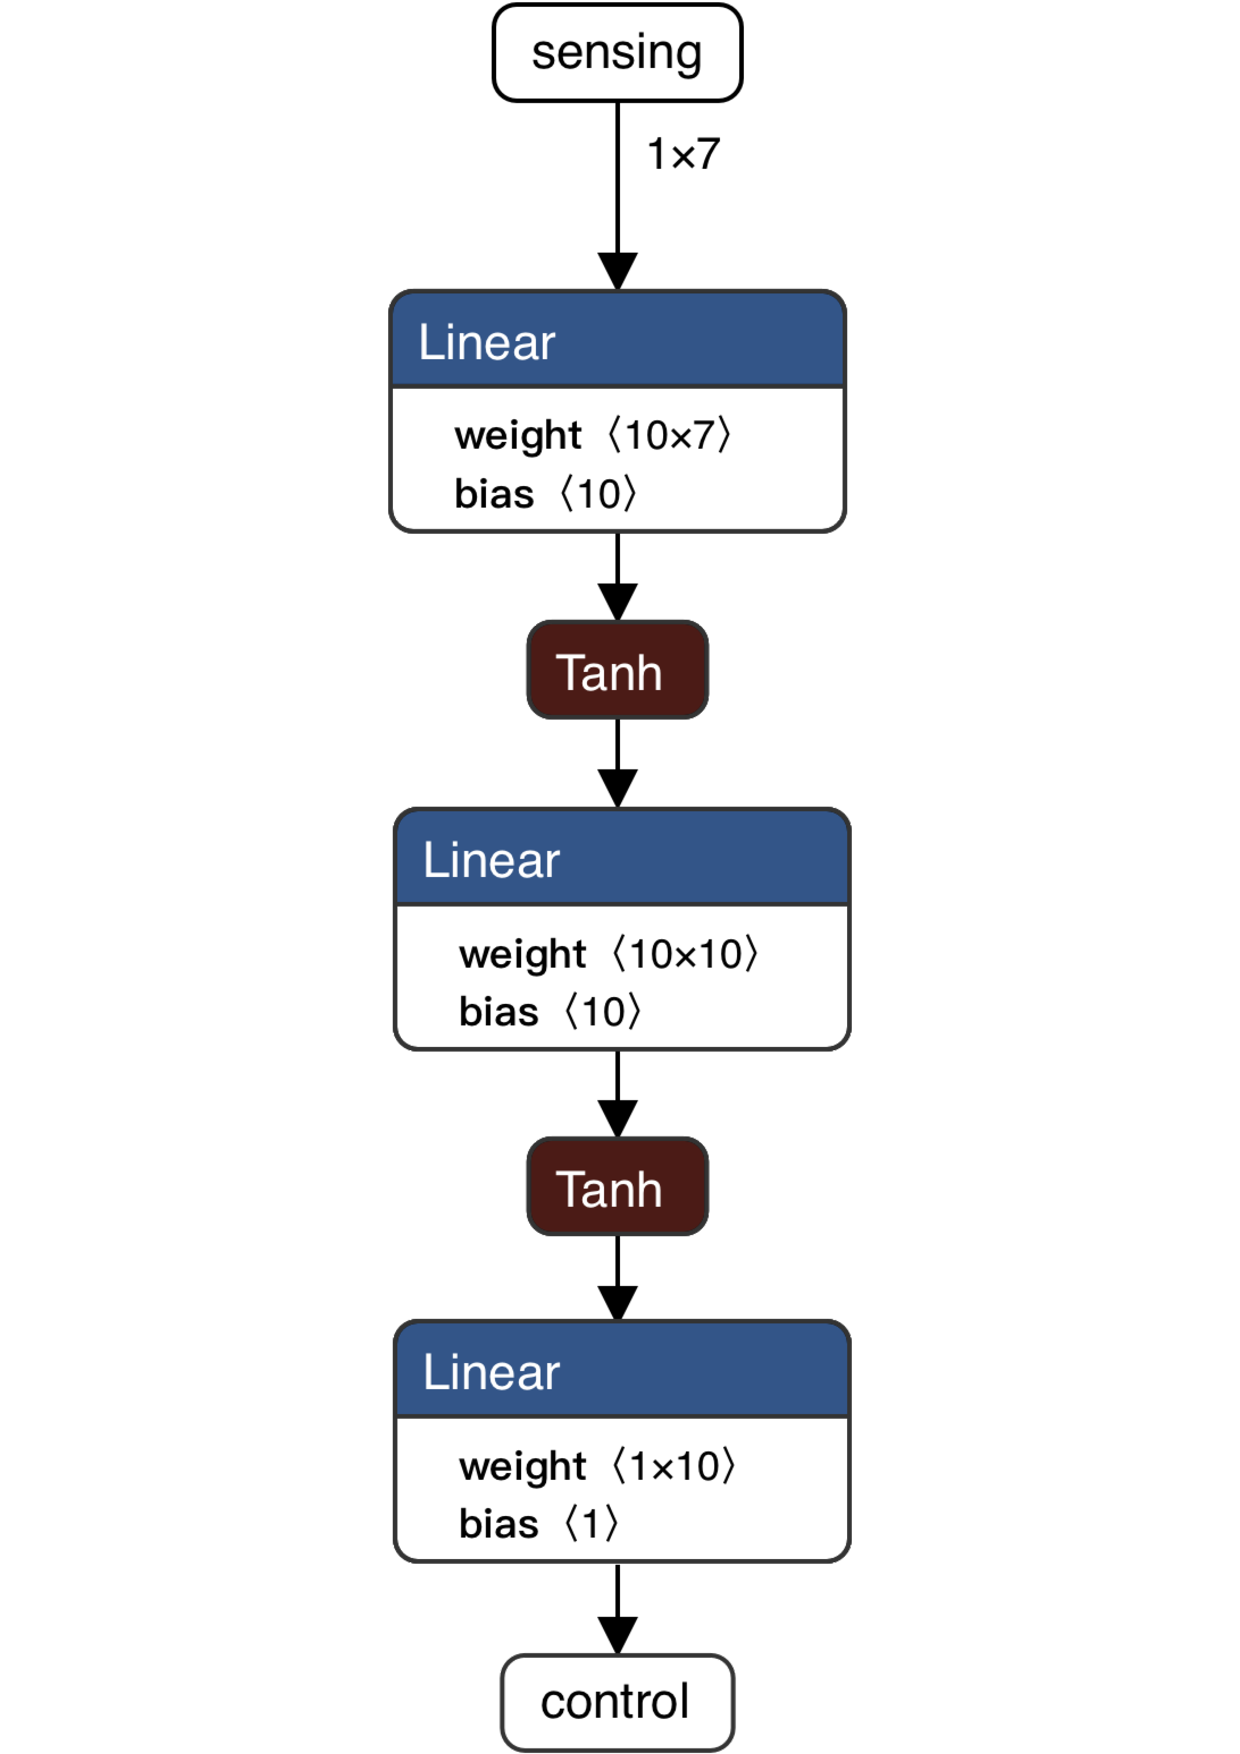
\includegraphics[width=.3\textwidth]{contents/images/task1distributed@4x}%
		\caption{Structure of a network with $7$ input sensing.}
		\label{fig:singlenet7distributed1}
	\end{subfigure}
	\hfill
	\begin{subfigure}[h]{0.495\textwidth}
		\centering
		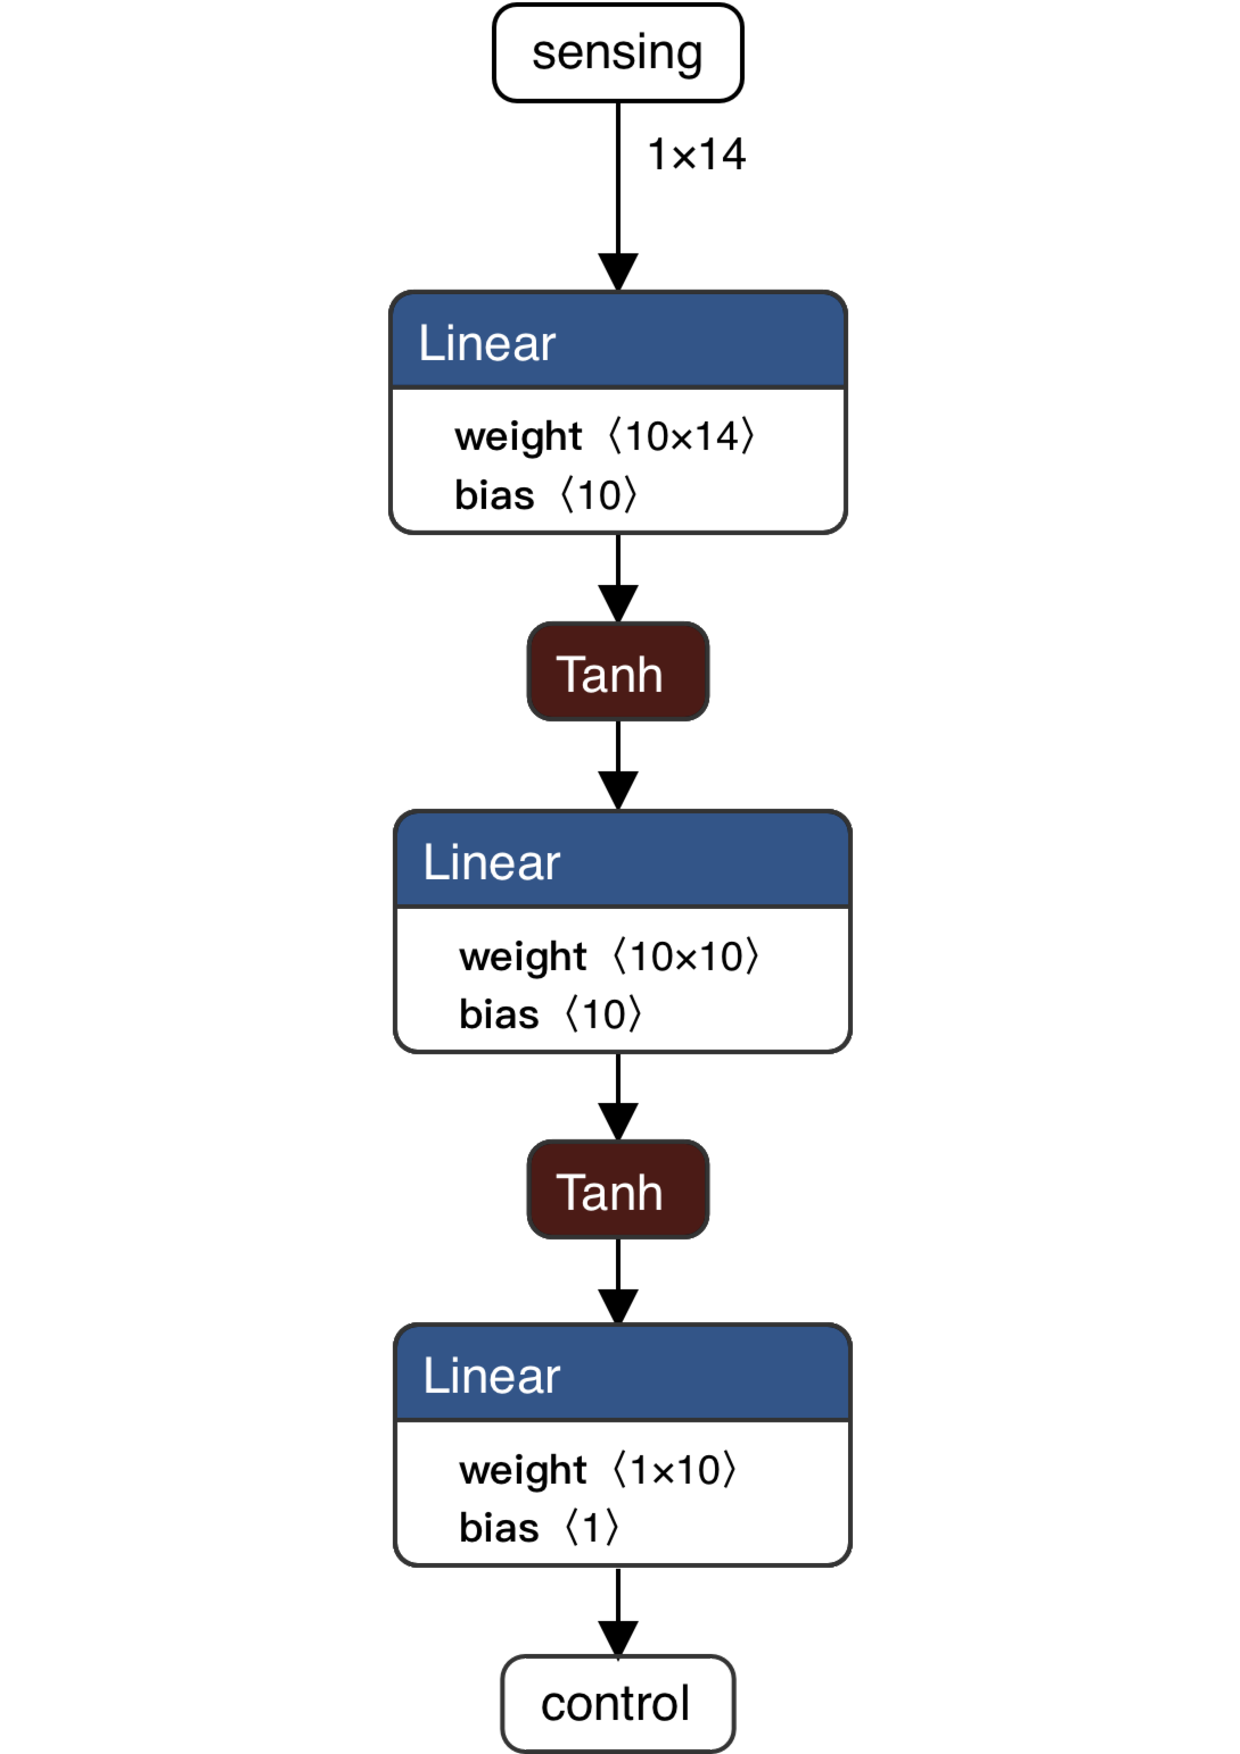
\includegraphics[width=.3\textwidth]{contents/images/task1distributed_all@4x}
		\caption{Structure of a network with $14$ input sensing.}
		\label{fig:singlenet14distributed1}
	\end{subfigure}
	\caption{Visualisation of the network architectures for the distributed 
		approach.}
	\label{fig:singlenetdistributed1}
\end{figure}

To the first and second layer is applied a non-linear activation function, 
useful to make the model generalise. 
In particular, we chose the hyperbolic tangent (Tanh) 
\cite[see][]{kalman1992tanh}, a zero-centred function, shown in Figure 
\ref{fig:tanh}, whose range lies between $[-1, 1]$ and its output is given by

\begin{Equation}[H]
	\centering
	\begin{equation}
	f(x)= \frac{\sinh (x)}{\cosh (x)} = \bigg( \frac{e^x - e^{-x}}{e^x + 
		e^{-x}}\bigg)
	\end{equation}
	\caption{Hyperbolic Tangent Function (Tanh).}
	\label{eq:tanh}
\end{Equation}

This type of activation function is often used in deep learning and one of is 
advantages is that negative inputs are mapped to strongly negative values.

\begin{figure}[htb]
	\centering
	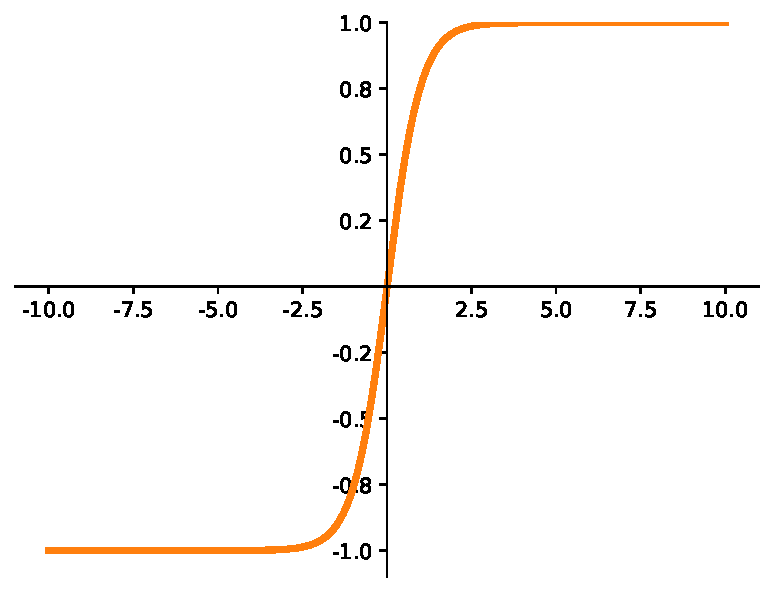
\includegraphics[width=.5\textwidth]{contents/images/tanh2}%
	\caption{Trend of the Tanh activation function.}
	\label{fig:tanh}
\end{figure}

%fixme citation
As optimiser we chose Adam, {an algorithm for first-order gradient-based 
optimisation of stochastic objective functions, based on adaptive estimates of 
lower-order moments}, \cite[see][]{kingma2014adam, 
loshchilov2017decoupled}, 
implemented in the \texttt{torch.optim} package, with a learning rate of $0.01$. 

Instead of computing the gradient descent on the entire dataset, the training set is 
split in mini-batches of size $100$ and an approximation of the gradient is 
produced, which makes the algorithm faster and at the same time, for sufficiently 
large numbers, the result is indistinguishable.

Gradient descent algorithms are susceptible to ``get stuck'' in local minima.
Mini-batches shuffle facilitate to avoid this problem by enabling the gradient to 
``bounce'' out of eventual local minimum, making it more variable by exploiting 
randomness, thereby helping convergence.

All the models are trained for $50$ epochs and evaluated using the \gls{mse} loss 
function, often used in regression problems. 
This criterion, implemented in the \texttt{torch.nn} package, measures the 
average of squared error between predictions and targets and learns to reduce it 
by penalising big errors in the model predictions.

\begin{Equation}[H]
	\centering
	\begin{equation}
	\mathtt{MSE} = \frac{\sum_{i=1}^n (y_i-\hat y_i)^2}{n}
	\end{equation}
	\caption{Mean Squared Error (\gls{mse}) loss function.}
	\label{eq:mse}
\end{Equation}
	
\subsubsection{...}
\label{subsubsec:....}


\subsection{Distributed approach experiments with communication}
\label{subsec:ex1comm}


\subsubsection{Learned controller}
\label{subsubsec:learnedcomm}
\subsection{Results}
\label{subsec:results1}

